\documentclass[12pt]{article}         
\usepackage{fullpage}
\usepackage[shortlabels]{enumitem}
\usepackage{amsmath}
\usepackage{amsfonts}
\usepackage{graphicx}
\graphicspath{ {./images/} }

%\usepackage{amsmath}
%\usepackage{amssymb}
%\usepackage{enumitem}

\title{CS250 Homework $\#$6}
\author{Sean O'Dea \footnote{Collaborated with Nobody.}}

\begin{document}
\maketitle

\section*{\textbf{1: P14.1.6} [8 pts]}
Prove that every language with a finite number of strings is the language of some DFA.


\subsection*{\textbf{Solution:}}
We know we can create a DFA for the empty language by looping all inputs on the start state (which is not a final state). \\

Assume for any language containing an arbitrary number of strings less than or equal to $n$ we can represent it with a DFA. \\

If we consider the same language with $n+1$ strings in it we must have concatenated a new letter onto the expression or added a letter to a union statement within the expression. It's important to note here that the regular expression defining a finite language cannot by definition contain any Kleene star statements. Because of this, we can represent any finite regular expression as a DFA that forms a line with the corresponding letter moves progressing to the right. Any non-accepted moves can go to a shared dead state. \\

If we have our existing DFA and a new letter is concatenated somewhere in the expression, we can add a state with one incoming edge and one outgoing edge in the corresponding place within the DFA as in the regular expression. If the letter is instead added to a union within the expression, we can just add an edge within the DFA between the same nodes the other letter goes between. This is similar to our algorithm for converting a regular expression to $\lambda$-NFA.\\

Any DFA containing an arbitrarily large but finite $n$ strings can be constructed in this way, therefore every language with a finite number of strings is the language of some DFA.


\newpage
\section*{\textbf{2: P14.2.4} [12 pts]}
A string in $\{a, \cdots , z\}^*$ is said to be \textbf{panalphabetic} if it contains at least one occurrence of each letter. Examples of panalphabetic strings are
$$thequickbrownfoxjumpsoverthelazydog$$ and $$jackdawslovemybigsphinxofquartz.$$ Is the language of panalphabetic strings decidable by a DFA? Prove your answer.


\subsection*{\textbf{Solution:}}
We can solve this by considering a simple case first. Let's consider an alphabet $\Sigma = \{ a, b \}$ with two distinct letters instead of 26. It's much simpler to construct a DFA for this example. We'll have 4 states: a start state $\iota$, a state where only $a$ has been seen, a state where only $b$ has been seen, and a final state where both $a$ and $b$ have been seen. \\

From the start state, an $a$ will bring you to the state where $a$ has been seen and a $b$ to the $b$ state. In either state if the same letter is seen it will just loop in that state. If the other letter is seen it will transition to the final state where all letters have now been seen at least once, confirming the string is panalphabetic. Below is a sketch of this DFA:

\begin{center}
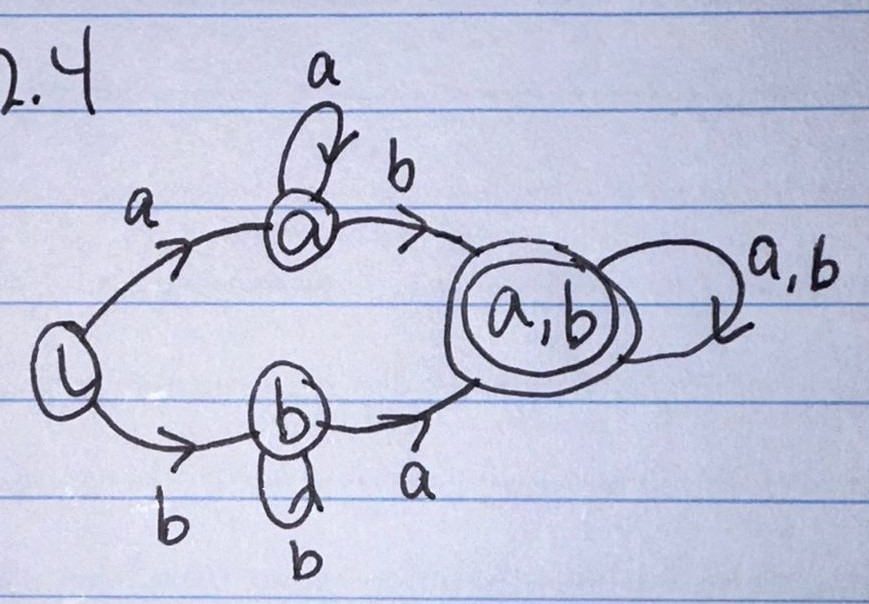
\includegraphics[scale=.2]{14.2.4.1}
\end{center}

Let's now look at a similar case but with the alphabet $\Sigma = \{ a, b, c \}$ which now has three distinct letters. We'll use the same logic to now contruct the larger DFA that handles three letters. Let's first construct our state list:

\[ \text{Previous states: } \{ (\iota), (a), (b), (a,b) \} \]
\[ \text{New states: } \{ (\iota), (a), (b), (c), (a,b), (a,c), (b,c), (a,b,c) \} \]

Each state represents the combination of letters which have already been seen. The final state will always be only the state which contains all letters of $\Sigma$. Below is a sketch of this larger DFA, notice that it directly builds on the previous DFA.

\begin{center}
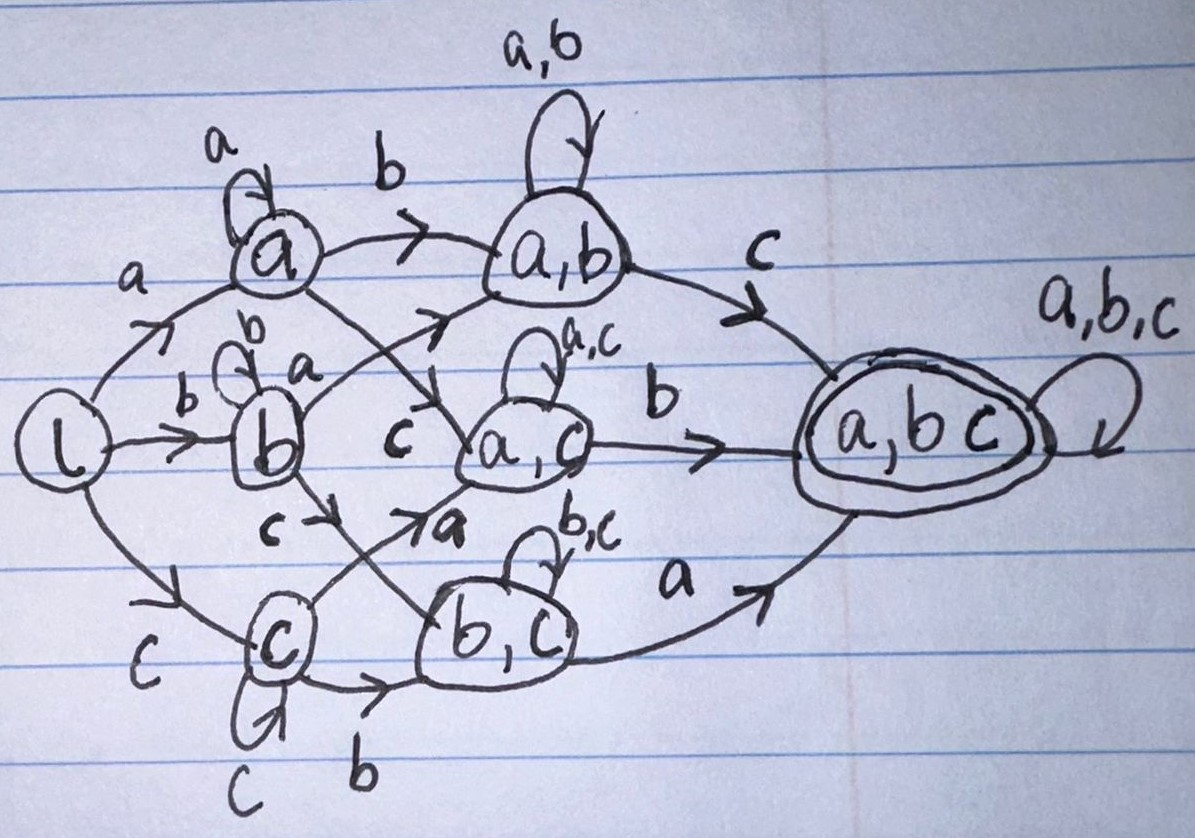
\includegraphics[scale=.2]{14.2.4.2}
\end{center}

For example's sake we'll look at the states of an alphabet with four letters but skip the sketch because it quickly gets large and complex. From our previous example we can imagine it would be built off of the previous DFA but now including the new letters moves and states.

\begin{multline*}
 \text{States for } \{ a, b, c, d \} \text{: } \{ (\iota), (a), (b), (c), (d), (a,b), (a,c), (a,d), (b,c), (b,d), (c,d), (a,b,c), \\
(a,b,d), (a,c,d), (b,c,d), (a,b,c,d) \}
\end{multline*}

We can continue this pattern by adding letters to the alphabet until we reach the 26 letters $a-z$ or any arbtirarily large finite alphabet. Thus, the language of panalphabetic strings is decidable by a DFA.

\newpage
\section*{\textbf{3: P14.3.6} [12 pts]}
Prove that the DFA from Exercise 14.3.6 is minimal, either by running the minimization algorithm on it or by showing that each pair of states is $L_5$-distinguishable.


\subsection*{\textbf{Solution:}}

This is what the initial DFA looks like based on the textbook's description:

\begin{center}
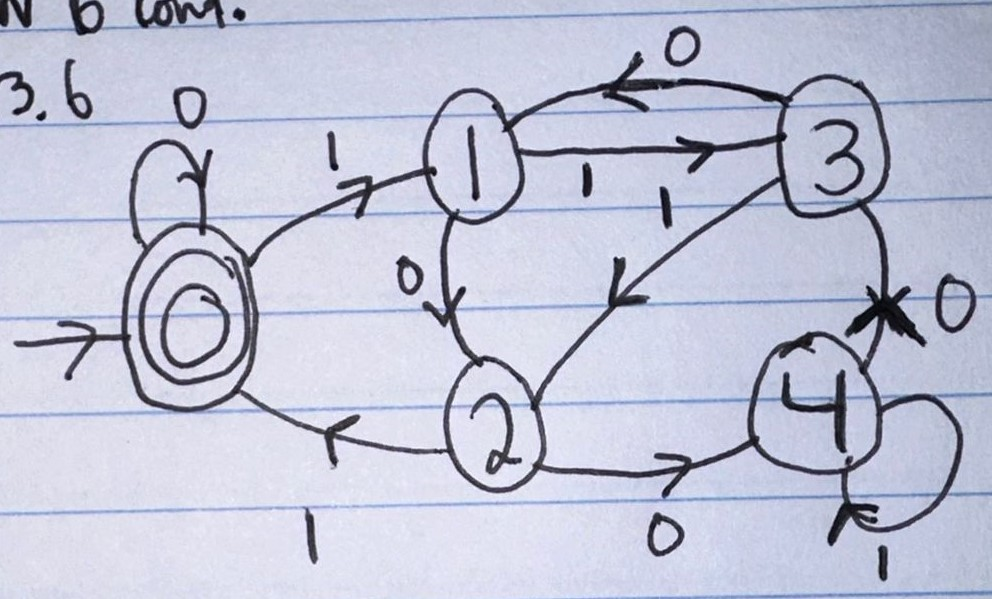
\includegraphics[scale=.25]{14.3.6}
\end{center}

Let's now apply the DFA minimization algorithm on it. We start by defining our first two equivalence classes, $F$ and $N$, representing the final and non-final states respectively. We know the $F$ class will remain alone the for the rest of the process because it's already in a class with only itself and there's no other final states in the DFA. Looking at the destinations of moves from each of the $N$-class nodes:

\begin{center}
\begin{tabular}{c | c c}
N & 0 & 1 \\
\hline
1 & N & N \\
2 & F & N \\
3 & N & N \\
4 & N & N \\
\end{tabular}
\end{center}

We can see the state that does not match the others is 2. Let's split it off into a separate class called $Y$ while the remaining states (minus 0) will be in a class called $X$. Repeating the process:

\begin{center}
\begin{tabular}{c | c c}
X & 0 & 1 \\
\hline
1 & Y & X \\
3 & X & Y \\
4 & X & X \\
\end{tabular}
\end{center}

We can see each of the states in the class $X$ are distinguishable from each other, and therefore must exist in their own respective equivalence classes. By this we've shown that all states in the original DFA are $L_5$-distinguishable and therefore the DFA is already in a minimized state.

\newpage
\section*{\textbf{4: P14.5.4} [15 pts]}
Let $N$ be an NFA with $k$ states. For every letter $a \in \Sigma$, define a $k$ by $k$ boolean matrix $M_a$ such that $M_a(i, j)$ is \texttt{true} if and only if $\langle i, a, j \rangle \in \Delta$. Define a function $f$ from $\Sigma^*$ to the set of $k$ by $k$ boolean matrices by the rules $f(\lambda) = I$, $f(wa) = f(w)M_a$. Prove that $w \in L(N)$ if and only if there is a final state $f$ such that the $(\iota, f)$ entry of $f(w)$ is \texttt{true}.



\subsection*{\textbf{Solution:}}
Proof that $w \in L(N) \implies $ there is a final state $f$ such that the $(\iota, f)$ entry of $f(w)$ is \texttt{true}:

We can prove this by induction on all strings $w \in \Sigma ^*$.

If $w = \lambda$, it will be in $L(N)$ if the start state is a final state. $f(\lambda)$ returns the identity matrix meaning we know $I(\iota, \iota)$ will be \texttt{true}, thus $I(\iota, f)$ will be $\texttt{true}$ if they're the same node.

Assume for some arbitrary string $w$, if $w \in L(N)$, there will be a final state $f$ such that the $(\iota, f)$ entry of $f(w)$ is \texttt{true}.

Let's now say we construct a string $w' = wa$ where $a$ is a letter in $\Sigma$. $w'$ will be in $L(N)$ if there is an edge to the final state using $a$ from the previous string. If this is the case we can use our hypothesis to multiply $f(w)M_a$ where $(\iota, f)$ of the result will be \texttt{true} if $(\iota, f)$ was true in $f(w)$ and $(f,f)$ is true in $M_a$. \\

\noindent
Proof that there is a final state $f$ such that the $(\iota, f)$ entry of $f(w)$ is \texttt{true} $\implies w \in L(N)$:

If $w = \lambda$, the $(\iota, f)$ entry of $f(w)$ will be \texttt{true} if $\iota$ is a final state because $f(\lambda) = I$. We know if $\iota$ is a final state this means the empty string is accepted by the NFA so $w \in L(N)$.

Assume for some arbitrary string $w$, if there is a final state $f$ such that the $(\iota, f)$ entry of $f(w)$ is \texttt{true}, then $w \in L(N)$.

Let's now say we construct a string $w' = wa$ where $a$ is a letter in $\Sigma$. The $(\iota, f)$ entry of $w$ determines whether it is in $L(N)$ by our hypothesis. If multiplication by $M_a$ results in a \texttt{false}, then $w'$ is not in $L(N)$, and if it results in \texttt{true} than $w'$ in in $L(N)$.


\newpage
\section*{\textbf{5: P14.6.9} [16 pts]}
Given a nonempty finite language $S$, consider the language $C_S = \Sigma^*S\Sigma^*$ of strings that have a substring in $S$.

\begin{enumerate}[(a)]
    \item Describe an ordinary NFA for this language. (Note: The Yes-$aba$ language is just $C_{\{aba\}}$.)
    \item Prove that in the minimal DFA for any such language $C_S$ has exactly one final state.
    \item Use the Subset Construction to find a DFA for the language $C_S$ where $S = \{aaa, bbb\}$. (You may invoke part (b) and not worry about distinguishing the different final states.
    \item Repeat part (c) for $S = \{abb, bab, bba\}$. Let $\Sigma = \{a, b\}$.
\end{enumerate}



\subsection*{\textbf{Solution:}}
\begin{enumerate}[(a)]
    \item Similar to 14.1.6, since $S$ is finite, we can represent it as a continuous contatenation. Also because it's nonempty there must be a path to some final state. For our ordinary NFA we can simply make a series of moves from $\iota$ to the final state with each move representing one letter being contatenated. If exactly one letter is concatenated it will be a single arrow to the next state. If a union is concatenated there will be parallel edges. (As mentioned earlier this is essentially the algorithm used to create a $\lambda$-NFA from a regular expression.) We can then loop the letters of $\Sigma$ on the start and final states.

For example, the Yes-$aba$ language can be represented simply by 4 states in a line, the first being the start and the last being the final state. The three edges in the middle will be $a$, $b$, and $a$ respectively. Then $a,b$ will loop on the final and start states. In the case of a general language $S$, the NFA representing $C_S$ will be the NFA for $S$ with $\Sigma$ looped on the start and final states.

    \item To prove this we want to show there is exactly one equivalence class where a string in $S$ is contained in the string. If we consider all strings that contain a string in $S$, they will all be \mbox{$C_S$-indistinguishable} because any strings concatenated on the end of them will not change the fact that they already contain something in $S$ and are therefore in the language. This means there must be only one equivalence class for strings contained in $C_S$.

    \item Before:

\begin{center}
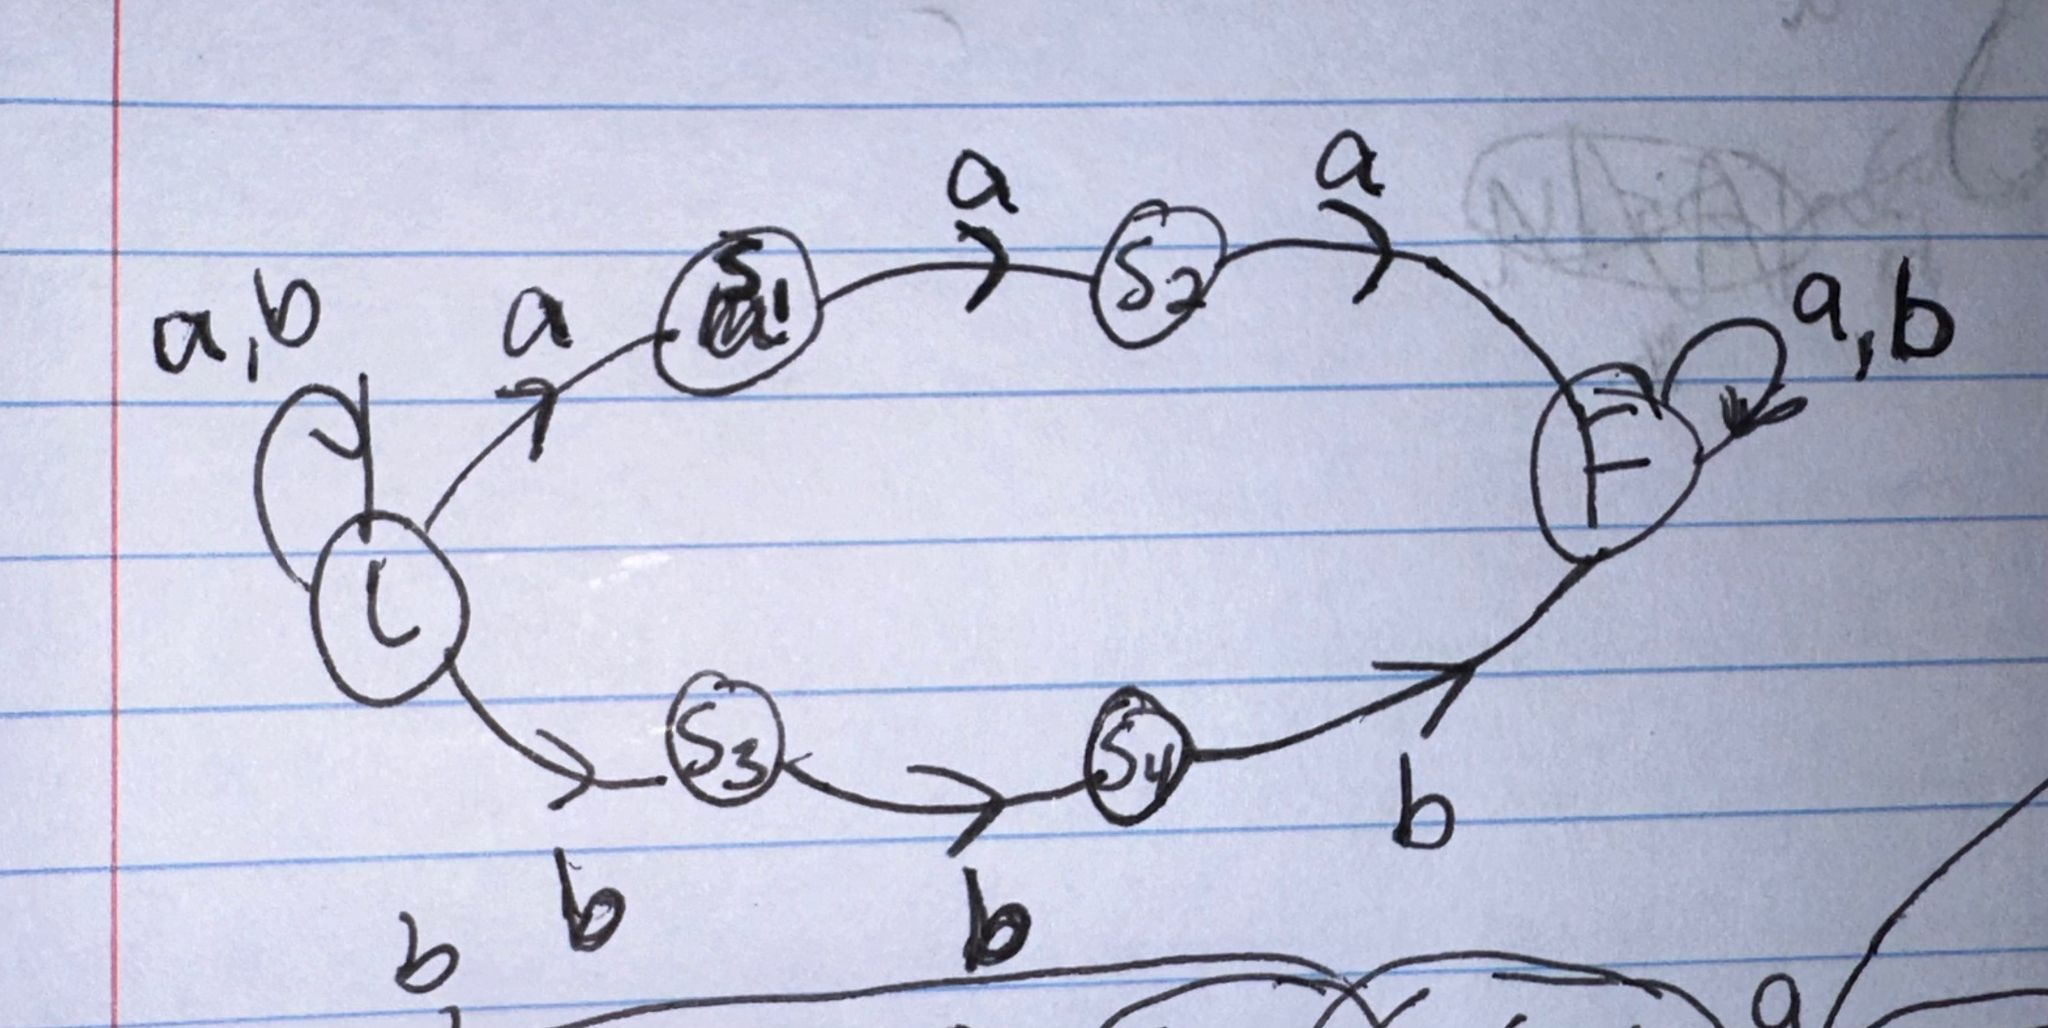
\includegraphics[scale=.1]{14.6.9.1}
\end{center}

After:

\begin{center}
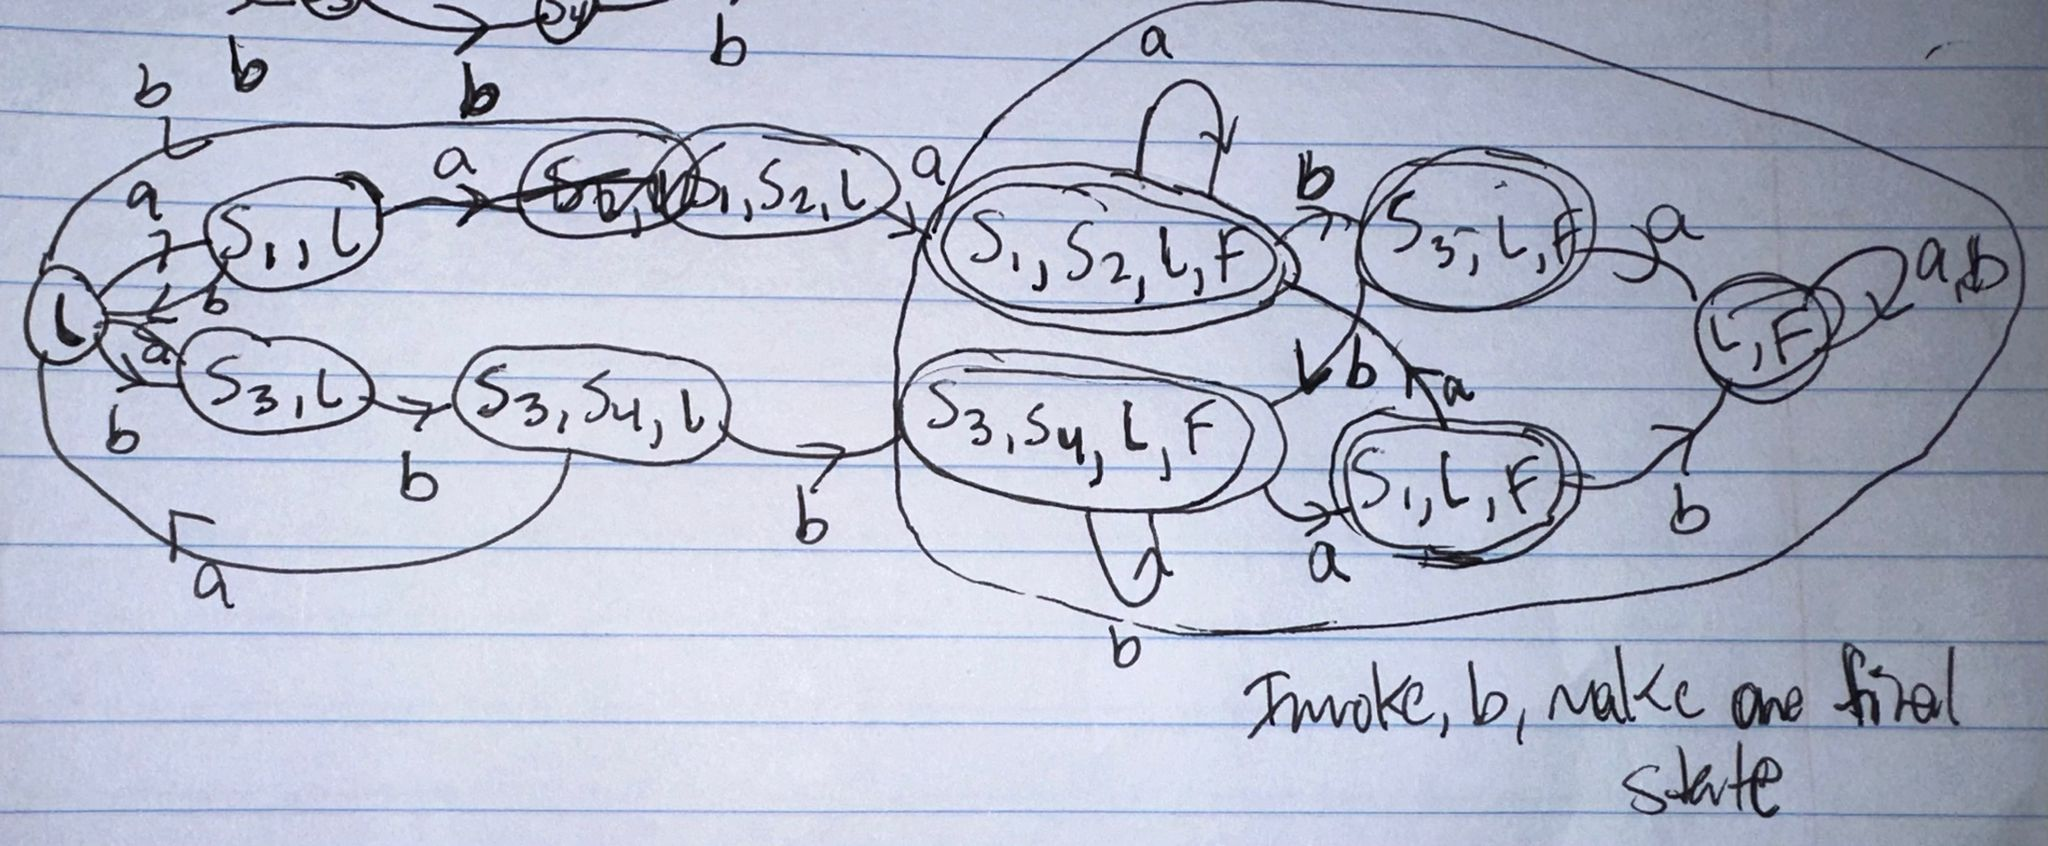
\includegraphics[scale=.15]{14.6.9.2}
\end{center}

    \item Before:

\begin{center}
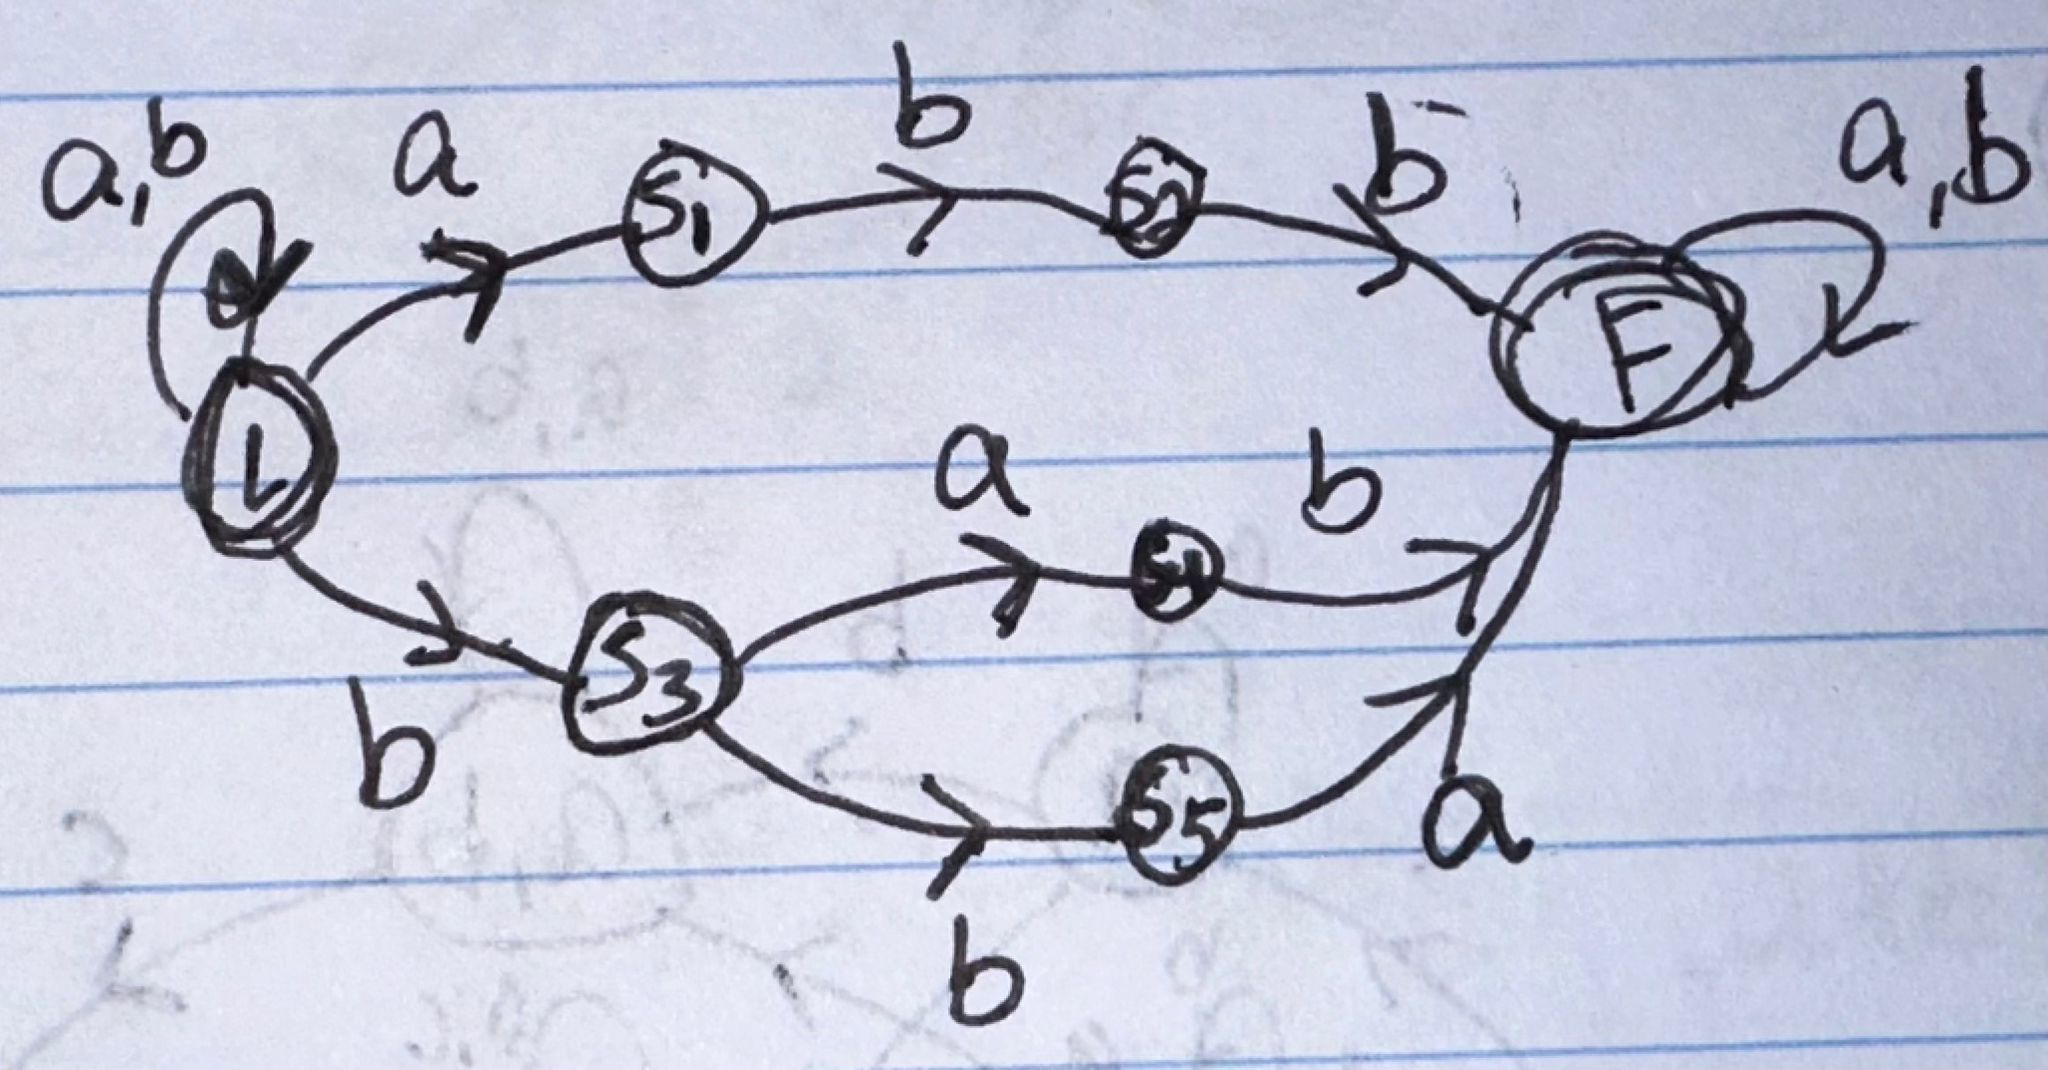
\includegraphics[scale=.1]{14.6.9.3}
\end{center}

After:

\begin{center}
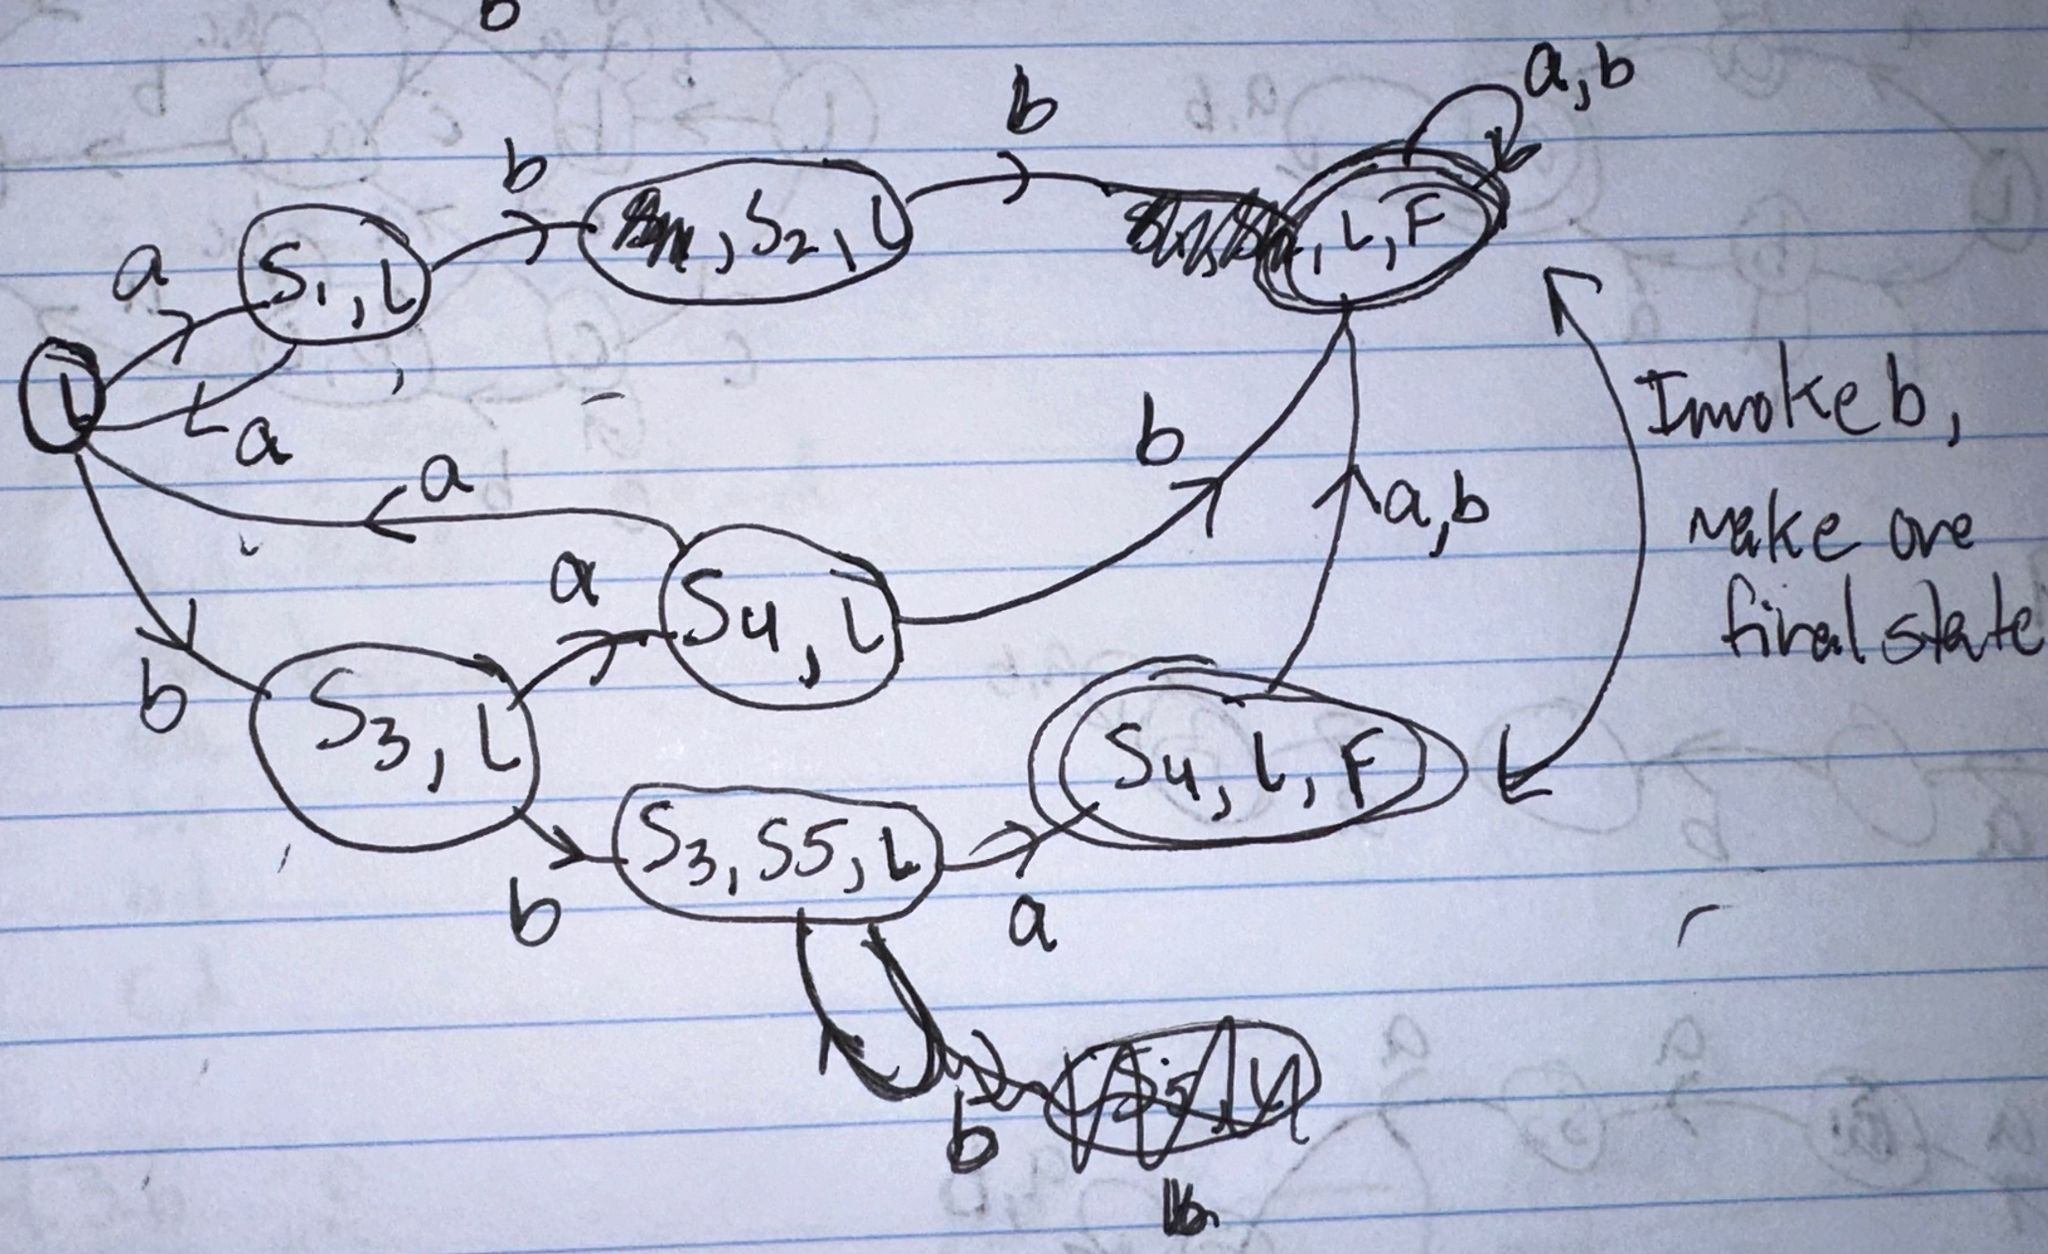
\includegraphics[scale=.15]{14.6.9.4}
\end{center}

\end{enumerate}


\newpage
\section*{\textbf{6: P14.7.6} [15 pts]}
Let $N$ be a $\lambda$-NFA in which there are two states $p$ and $q$ with transitions $\langle p, \lambda, q \rangle$ and $\langle q, \lambda, p \rangle$. Show that there is a $\lambda$-NFA $N'$, with $L(N') = L(N)$, such that $N'$ has a single state $r$ instead of $p$ and $q$. Should $r$ be a final state? What if $p$ or $q$ is the start state? What should be the transitions in and out of $r$? Should any other transitions from $N$ change? Prove that with your choices, $L(N) = L(N')$.


\subsection*{\textbf{Solution:}}
Using killing $\lambda$-move on only states $p$ and $q$ we can combine them into a single state $r$. When we do this we see that any edge coming into $p$ and then to $q$ by $\lambda$, and vice versa, can be combined into one edge. Because there's a $\lambda$ edge between the two in both directions we can move between them interchangeably. This is the reason we can combine the states. If there was an edge into $p$, then to $q$ by $\lambda$, then out of $q$, we can eliminate the $\lambda$-move in the middle. This goes both directions.\\

The properties of the combined state $r$ will depend on the previous properties of $p$ and $q$. $r$ will only be a final state if $p$ or $q$ are final. $r$ will be a start state only if $p$ or $q$ were a start state. The transitions in and out of $r$ will correspond to the edges originally coming in and out of $p$ and $q$. \\

We can check the validity of these parameters. If we think about the NFA $N$, if either $p$ or $q$ was a start state, we could have moved to the other state by a $\lambda$-move, leaving us in the same position in the string and now starting on the other state. If either $p$ or $q$ was a final state, we could have moved from our current state to the final one by a $\lambda$-move, meaning effectively both $p$ and $q$ can be final states. And having our transitions as described above follows from the killing $\lambda$-move algorithm, but only used on $p$ and $q$ this time. \\

With these rules the language $N$ will remain unchanged and therefore $L(N) = L(N')$.


\newpage
\section*{\textbf{7: P14.8.7} [12 pts]}
In Section 5.5 we gave a recursive algorithm that decides whether the language of a given regular expression is empty.
\begin{enumerate}[(a)]
    \item  Prove that if $N$ is a $\lambda$-NFA obeying our three rules, $L(N) = \emptyset$ if and only if there is no path from the start state to the final state in $N$.

    \item Prove, by induction on all regular expressions $\alpha$, that the emptiness tester of Section 5.5 returns \texttt{false} on input $\alpha$ if and only if the $\lambda$-NFA constructed from $\alpha$ has a path from the start state to the final state.
\end{enumerate}


\subsection*{\textbf{Solution:}}

\begin{enumerate}[(a)]
    \item  Our three rules are as follows:

\begin{enumerate}[1.)]
	\item There's exactly one final state (that's also not the start state).
	\item There are no outgoing edges from the final state.
	\item There are no incoming edges into the start state.
\end{enumerate}

    	Assume we have some $\lambda$-NFA $N$ obeying these three rules with a path to the final state from the start state. This means there must be some number of character moves (including $\lambda$) that can get to the final state. We also know the final state isn't the start state so there must be at least one move. This means $L(N)$ cannot be empty if the path exists because it contains at least $\lambda$ or a single character. By contrapositive this proves, $L(N) = \emptyset \implies $ No path. \\ 

Let's now prove the inverse. Now assume $N$ has no path from the start state to the final state. We know the start state is not final by our rules. Thus, there is no string that can let us reach an accepted state (including $\lambda$), so the language must be empty in this case. This proves, No path $\implies L(N) = \emptyset$. We've now proven both sides of the implication from the statement above.

\item Proof that \texttt{emptyLanguage($\alpha$)} returns \texttt{false} $\implies$ Path from start to final :

If $\alpha = \emptyset$ the function's base case will return \texttt{false}. This mean's the language is empty and there is no path by Part a.

Assume for some arbitrary regular expression $\alpha$ if the function returns \texttt{false}, there exists a path from the start to final state.

Let's say we construct a new regular expression from $\alpha$ called $\alpha '$. 

If $\alpha '$ = $(\alpha )*$ the function will return \text{false} if $\alpha$ is nonempty. Taking the Kleene star of an nonempty language will be nonempty and thus there will be a path to the final by Part a.

If $\alpha '$ = $\alpha w$ where $w \in \Sigma$ the function will return \texttt{true} either way because the language now contains at least $w$. This means the path exists because it will be at least a move with the one character to the final state.

If $\alpha '$ = $\alpha + \beta$ where $\beta$ is some other valid regular expression, the function will return \texttt{false} if either of the expressions are nonempty by our hypothesis. In this case a path must exist to the final by Part a. \\

Proof that Path from start to final $\implies$ \texttt{emptyLanguage($\alpha$)} returns \texttt{false} :

If $\alpha$ is nonempty there is path to the final by Part a, and the function returns \texttt{false}.

Assume for some arbitrary regular expression $\alpha$ if there exists a path from the start to final state, the function returns \texttt{false}.

Let's say we construct a new regular expression from $\alpha$ called $\alpha '$. 

If $\alpha '$ = $(\alpha )*$ there will exist a path to the final if $\alpha$ is nonempty so the function will return \texttt{false} by our hypothesis.

If $\alpha '$ = $\alpha w$ where $w \in \Sigma$ there must exist a path to the final because the language is now nonempty (it was concatenated with a letter or $\lambda$). So the function will return \texttt{false}.

If $\alpha '$ = $\alpha + \beta$ where $\beta$ is some other valid regular expression, there will exist a path if either $\alpha$ or $\beta$ are nonempty, in which case the function returns \texttt{false}.

\end{enumerate}


\newpage
\section*{\textbf{8: P14.10.3 - Variant} [10+5 extra pts]}
Find a regular expression for the language of strings in $\{a, b\}^*$ whose number of $a$’s and number of $b$’s are \textbf{congruent} modulo 3. (Hint: Build a DFA and use state elimination. This gets a bit messy. The problem in the textbook has the number of $a$’s and the number of $b$'s \textit{both} divisible by 3. We’ll give you five extra points for solving the original version.)


\subsection*{\textbf{Solution:}}
For the intial DFA, I used 9 states. Each state is labeled with two digits, the left being the number of $a$'s mod 3 and the right being the number of $b$'s mod 3. The original final states are the middle diagonal of the automota, states 00, 11, and 22. I later made a separate start and final state as our algorithm describes. My state elimination process was as follows:

\begin{figure} [!h]
	\centering
	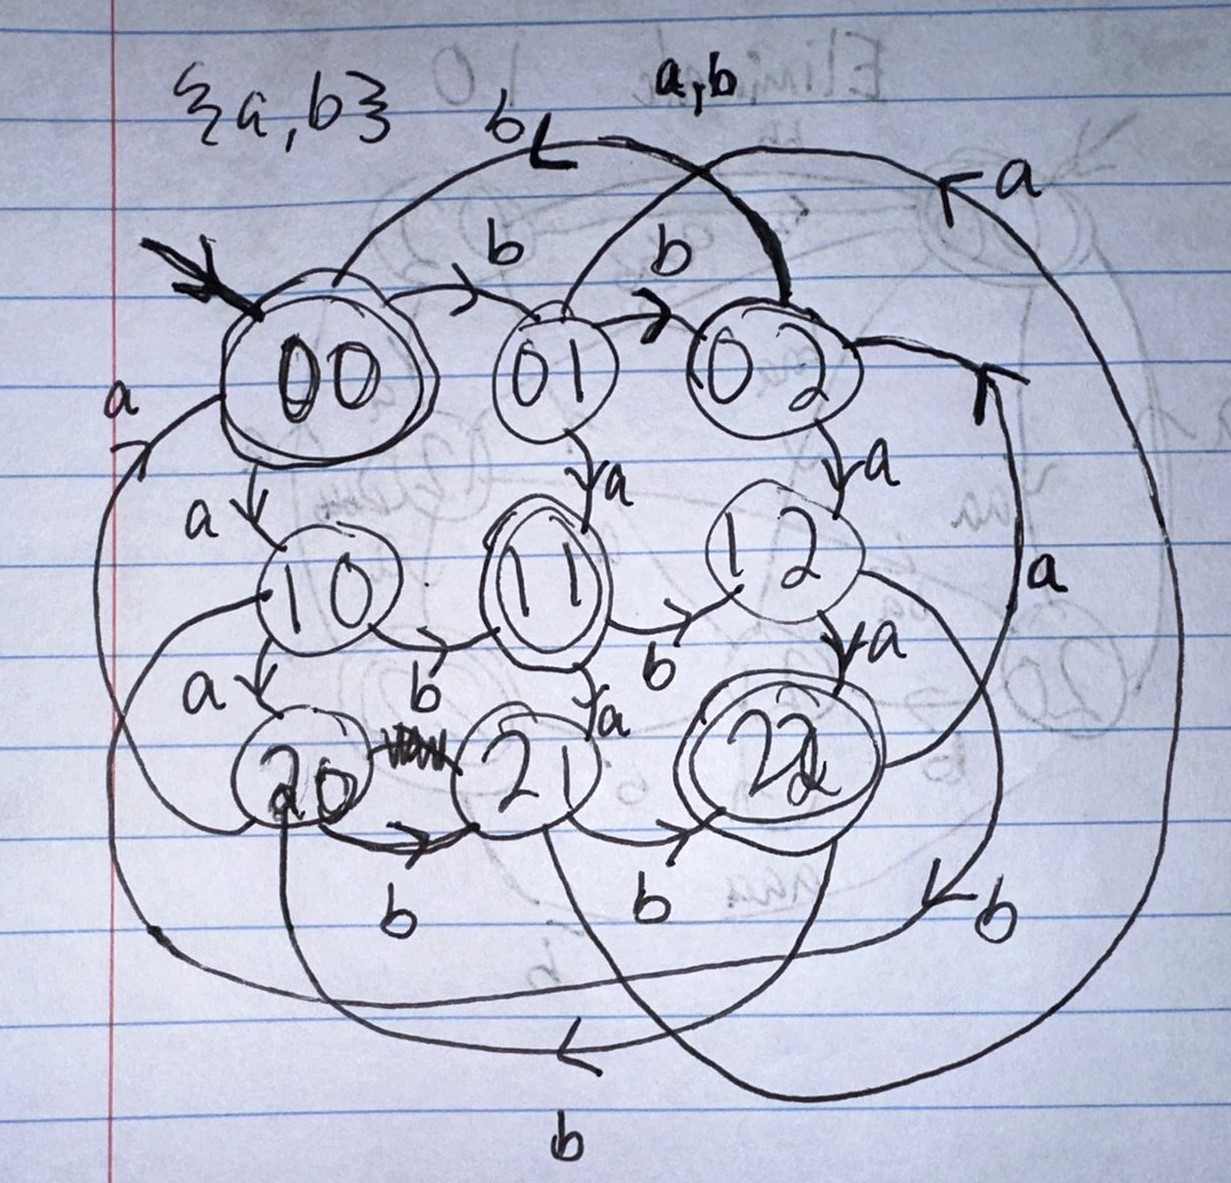
\includegraphics[scale=.2]{14.10.3.1}
	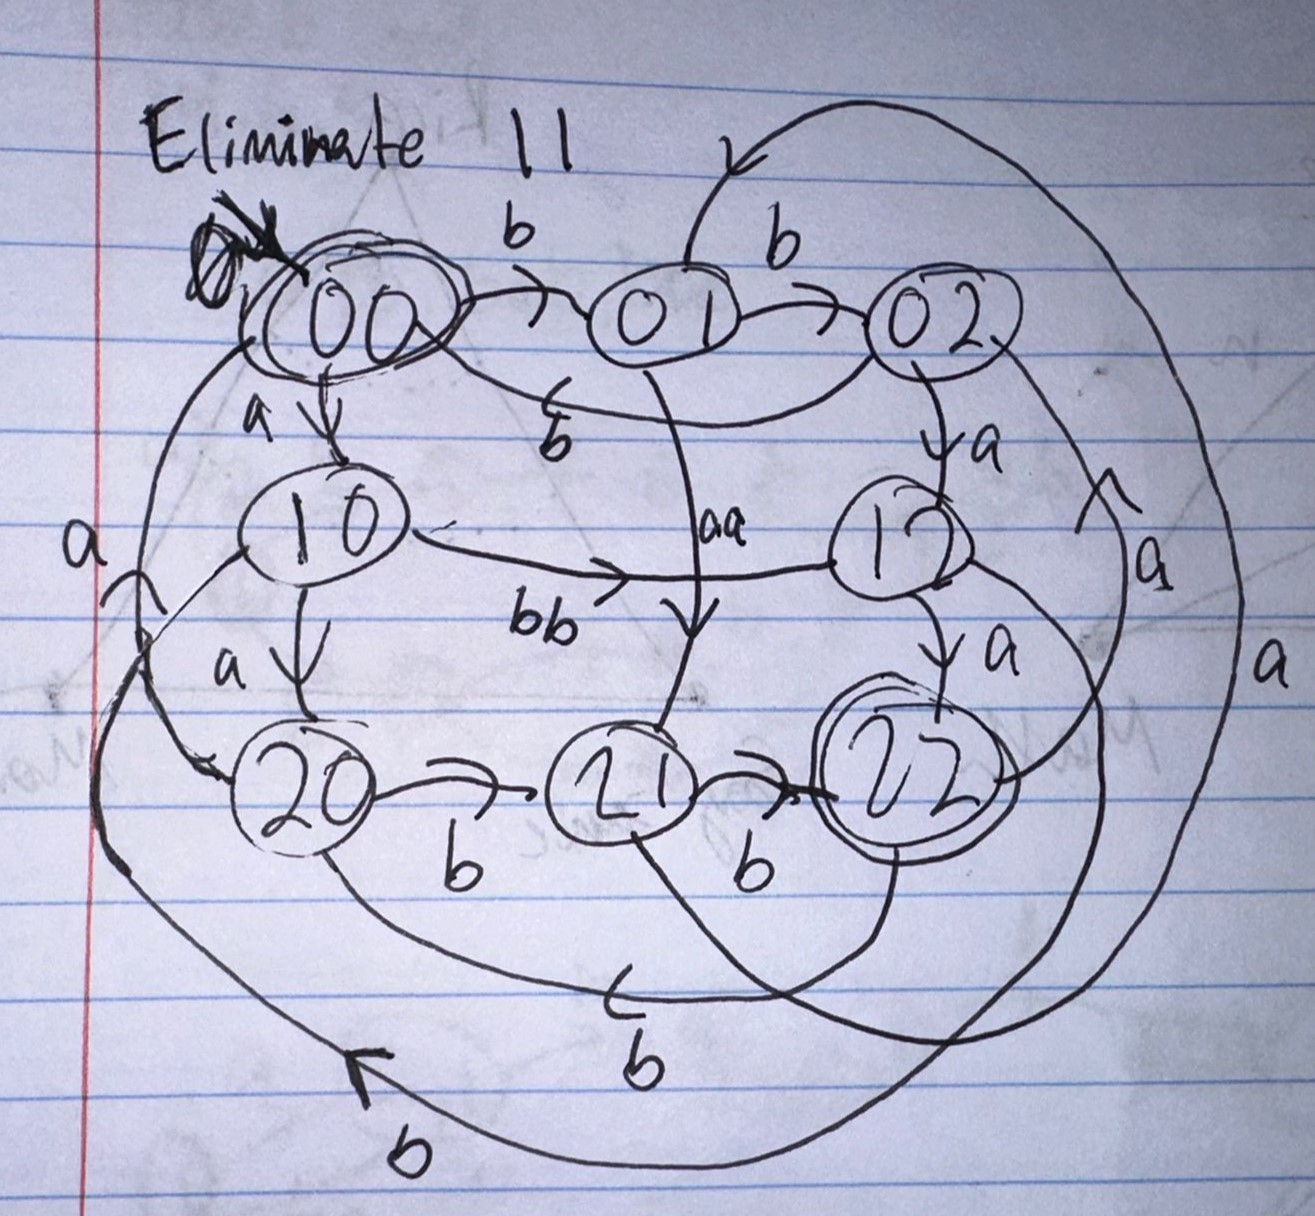
\includegraphics[scale=.2]{14.10.3.2}
\end{figure}

\begin{figure} [!h]
	\centering
	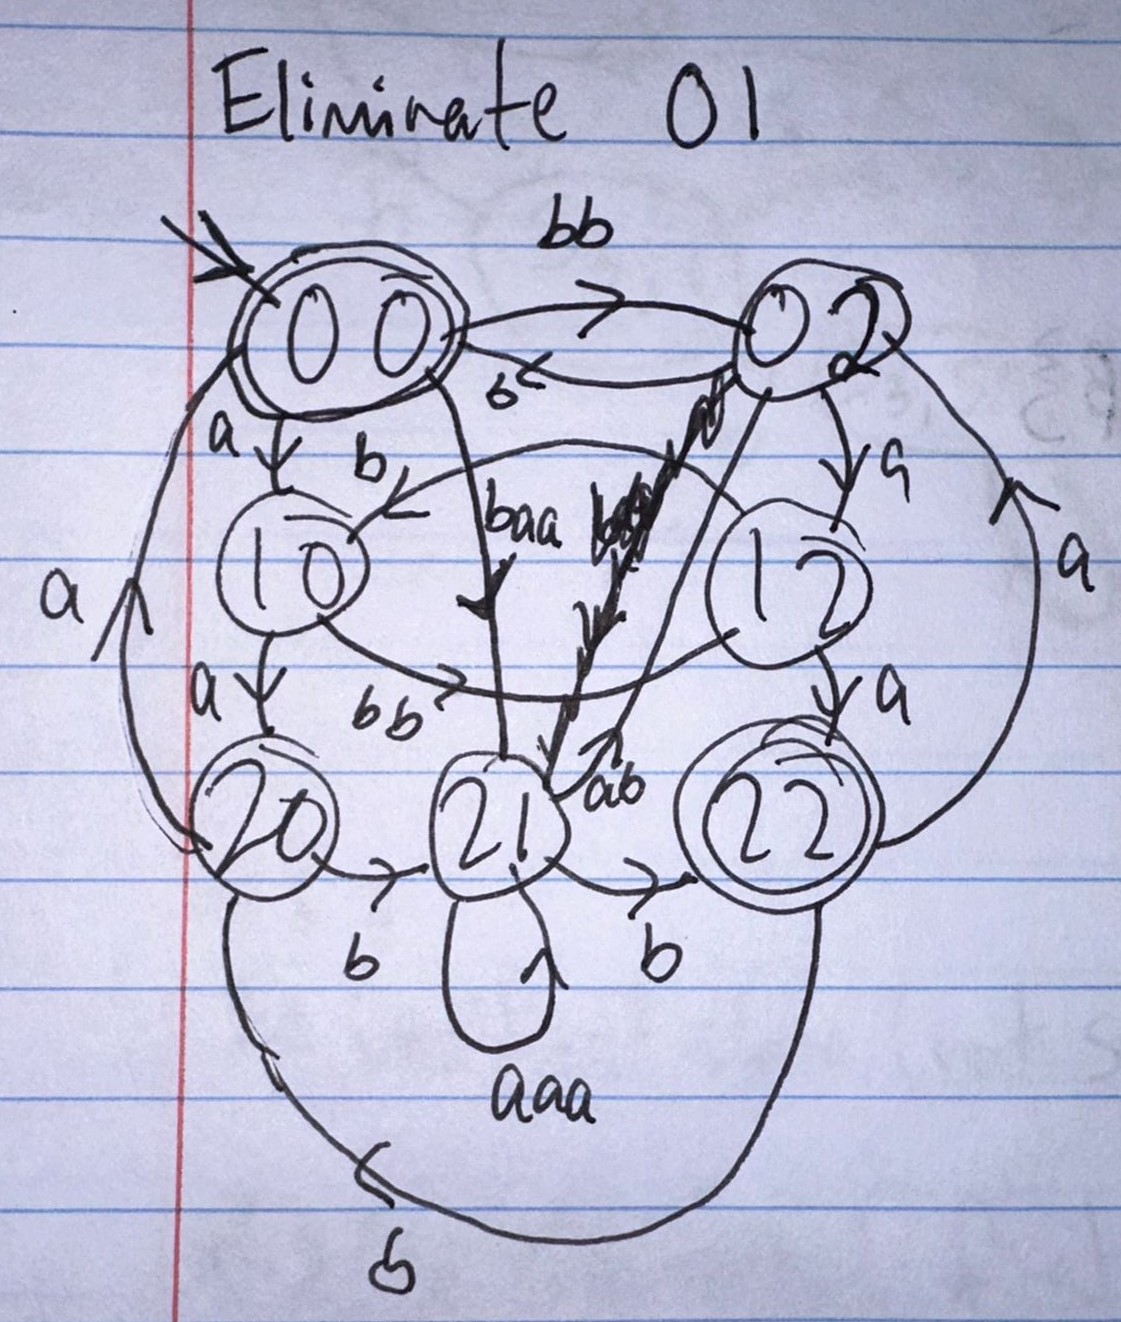
\includegraphics[scale=.2]{14.10.3.3}
	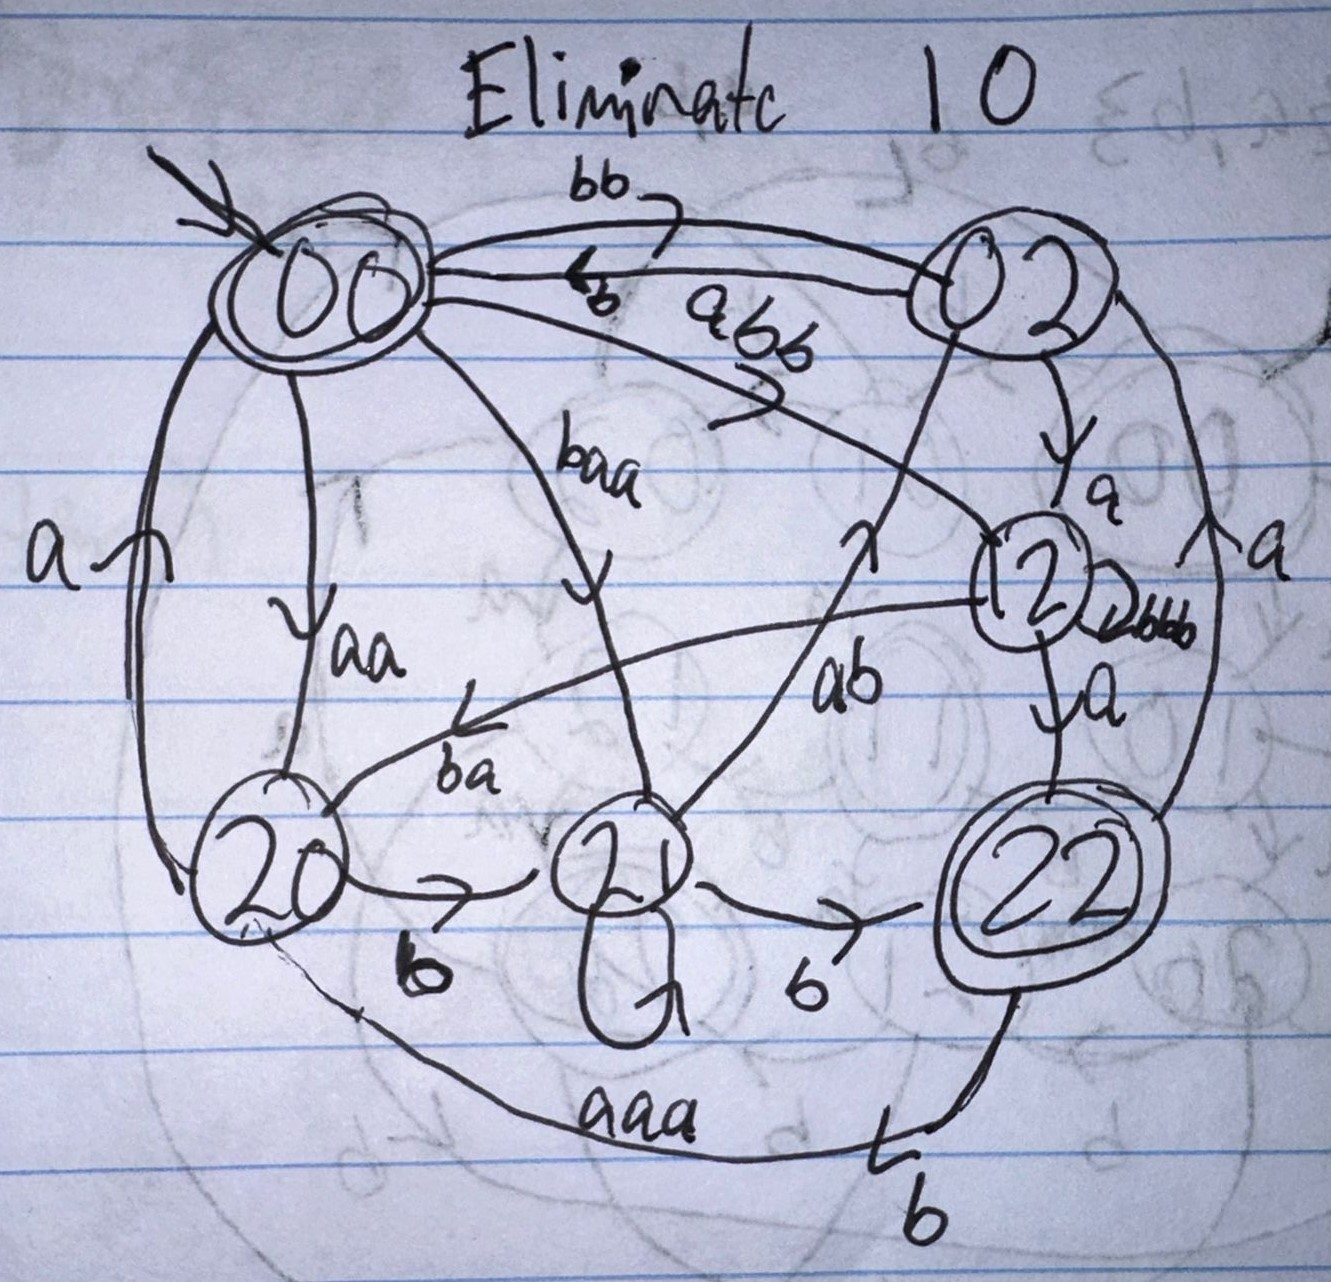
\includegraphics[scale=.2]{14.10.3.4}
\end{figure}

\begin{figure} [!h]
	\centering
	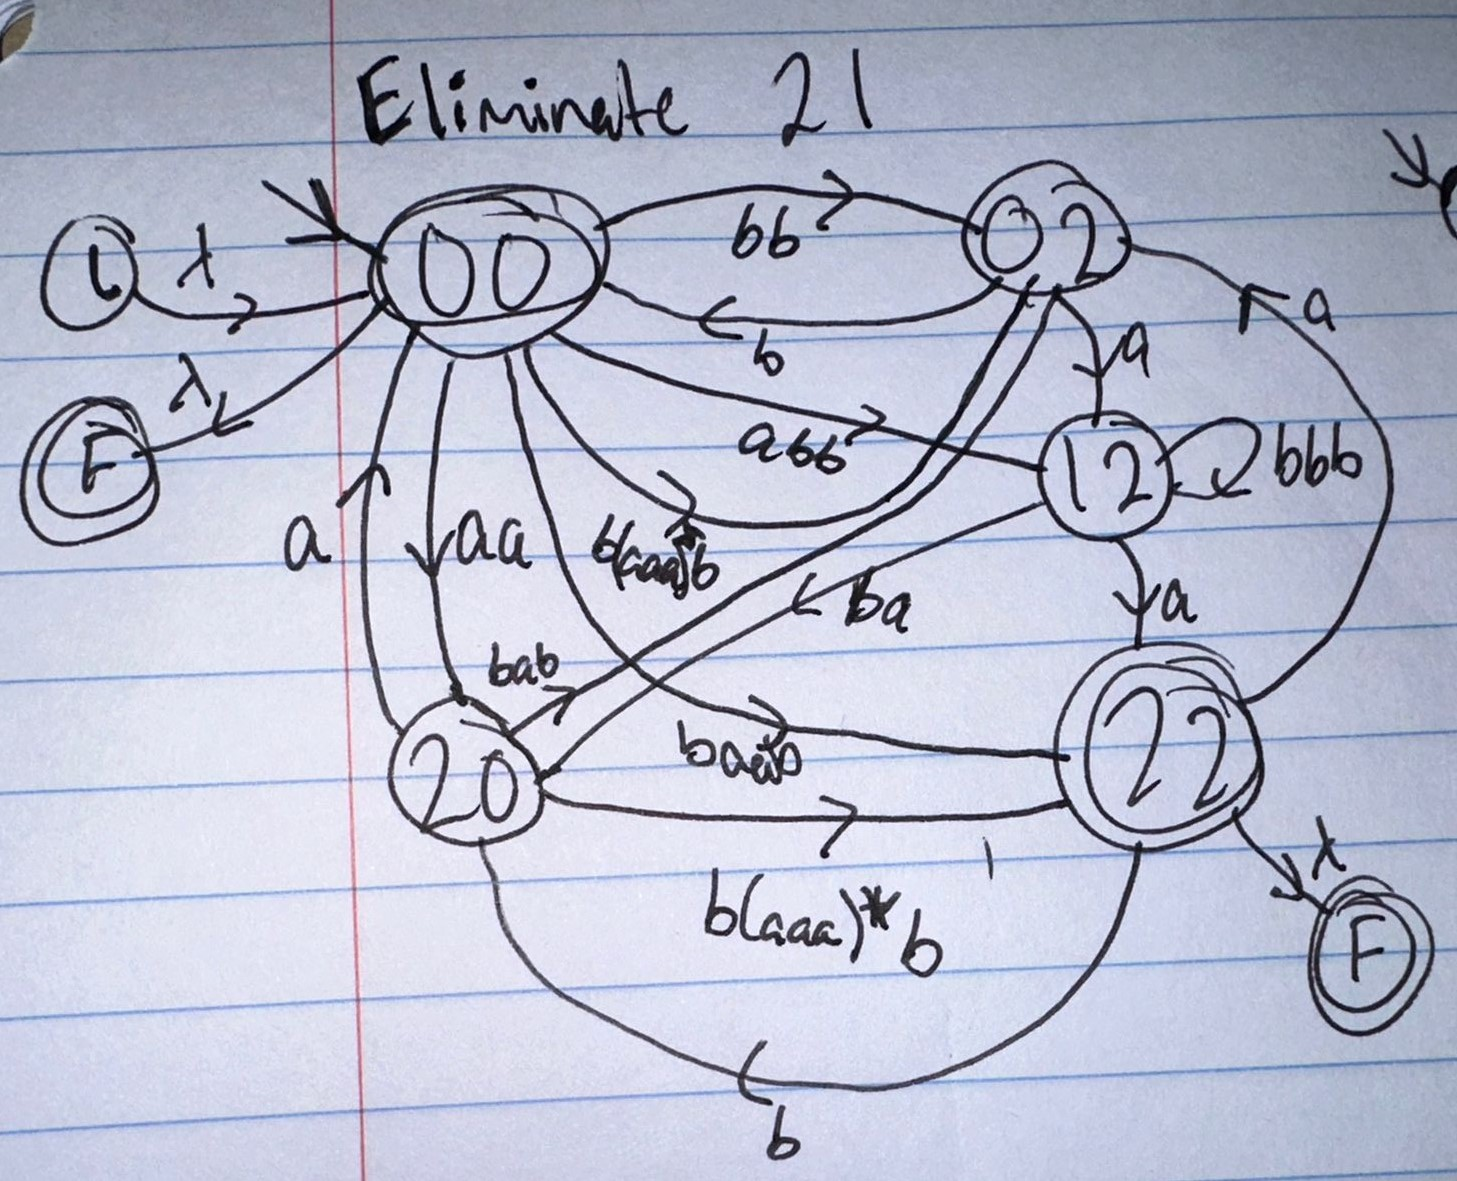
\includegraphics[scale=.2]{14.10.3.5}
	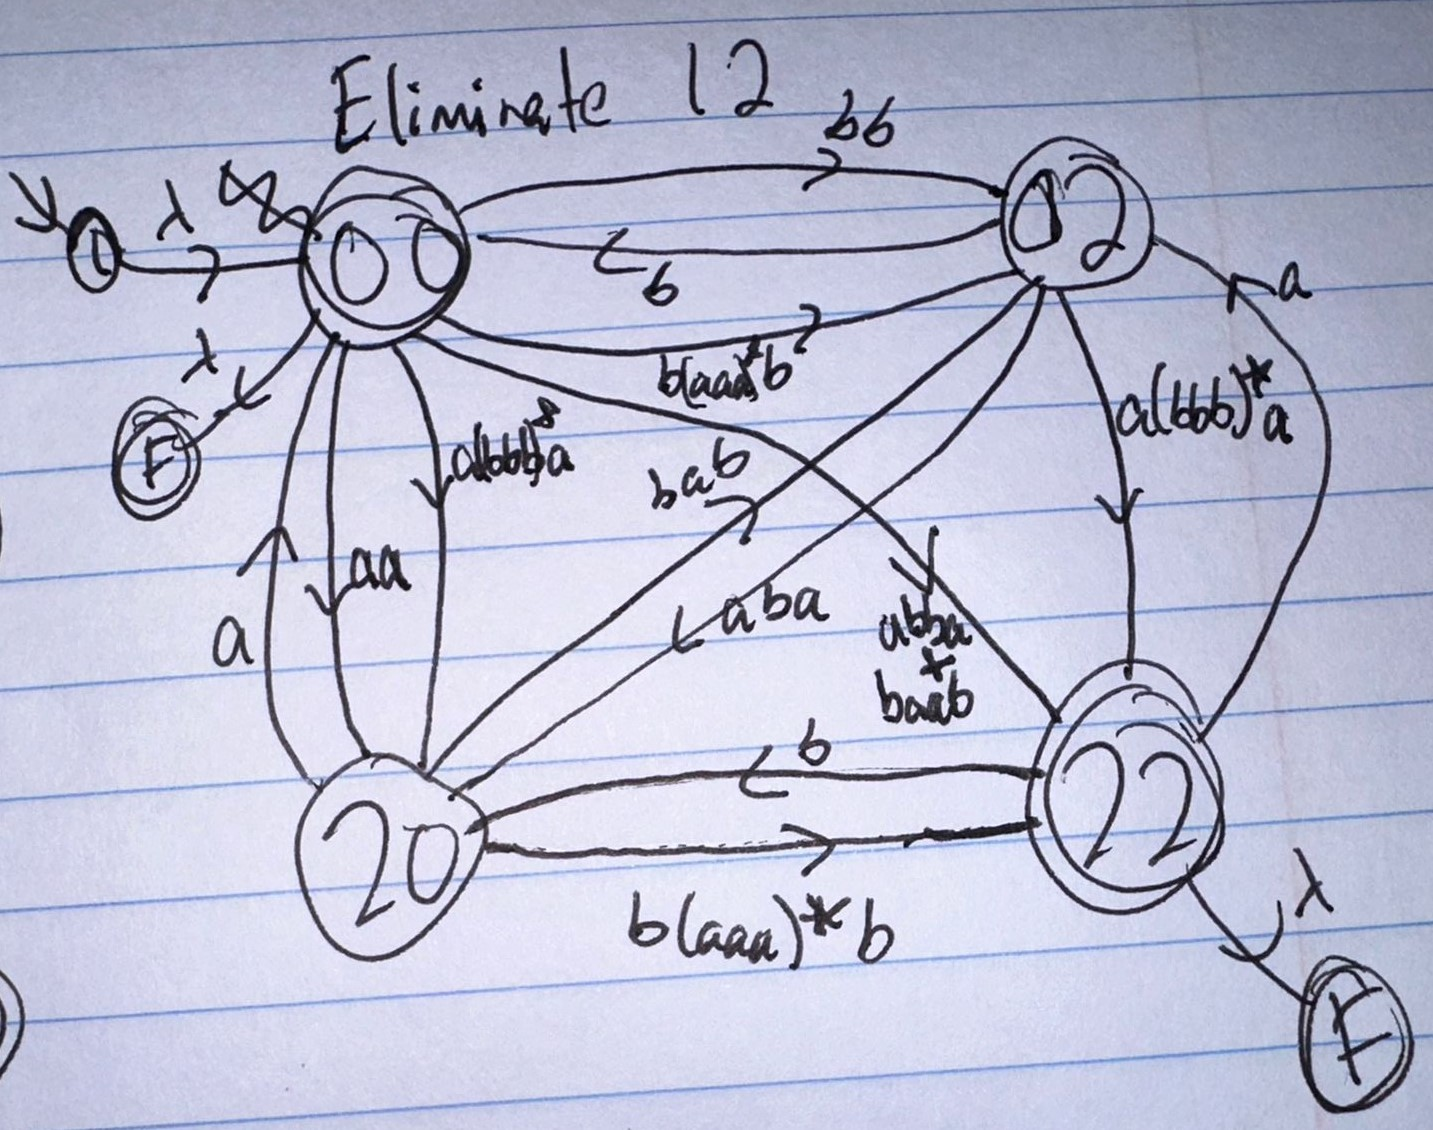
\includegraphics[scale=.2]{14.10.3.6}
\end{figure}

\begin{figure} [!h]
	\centering
	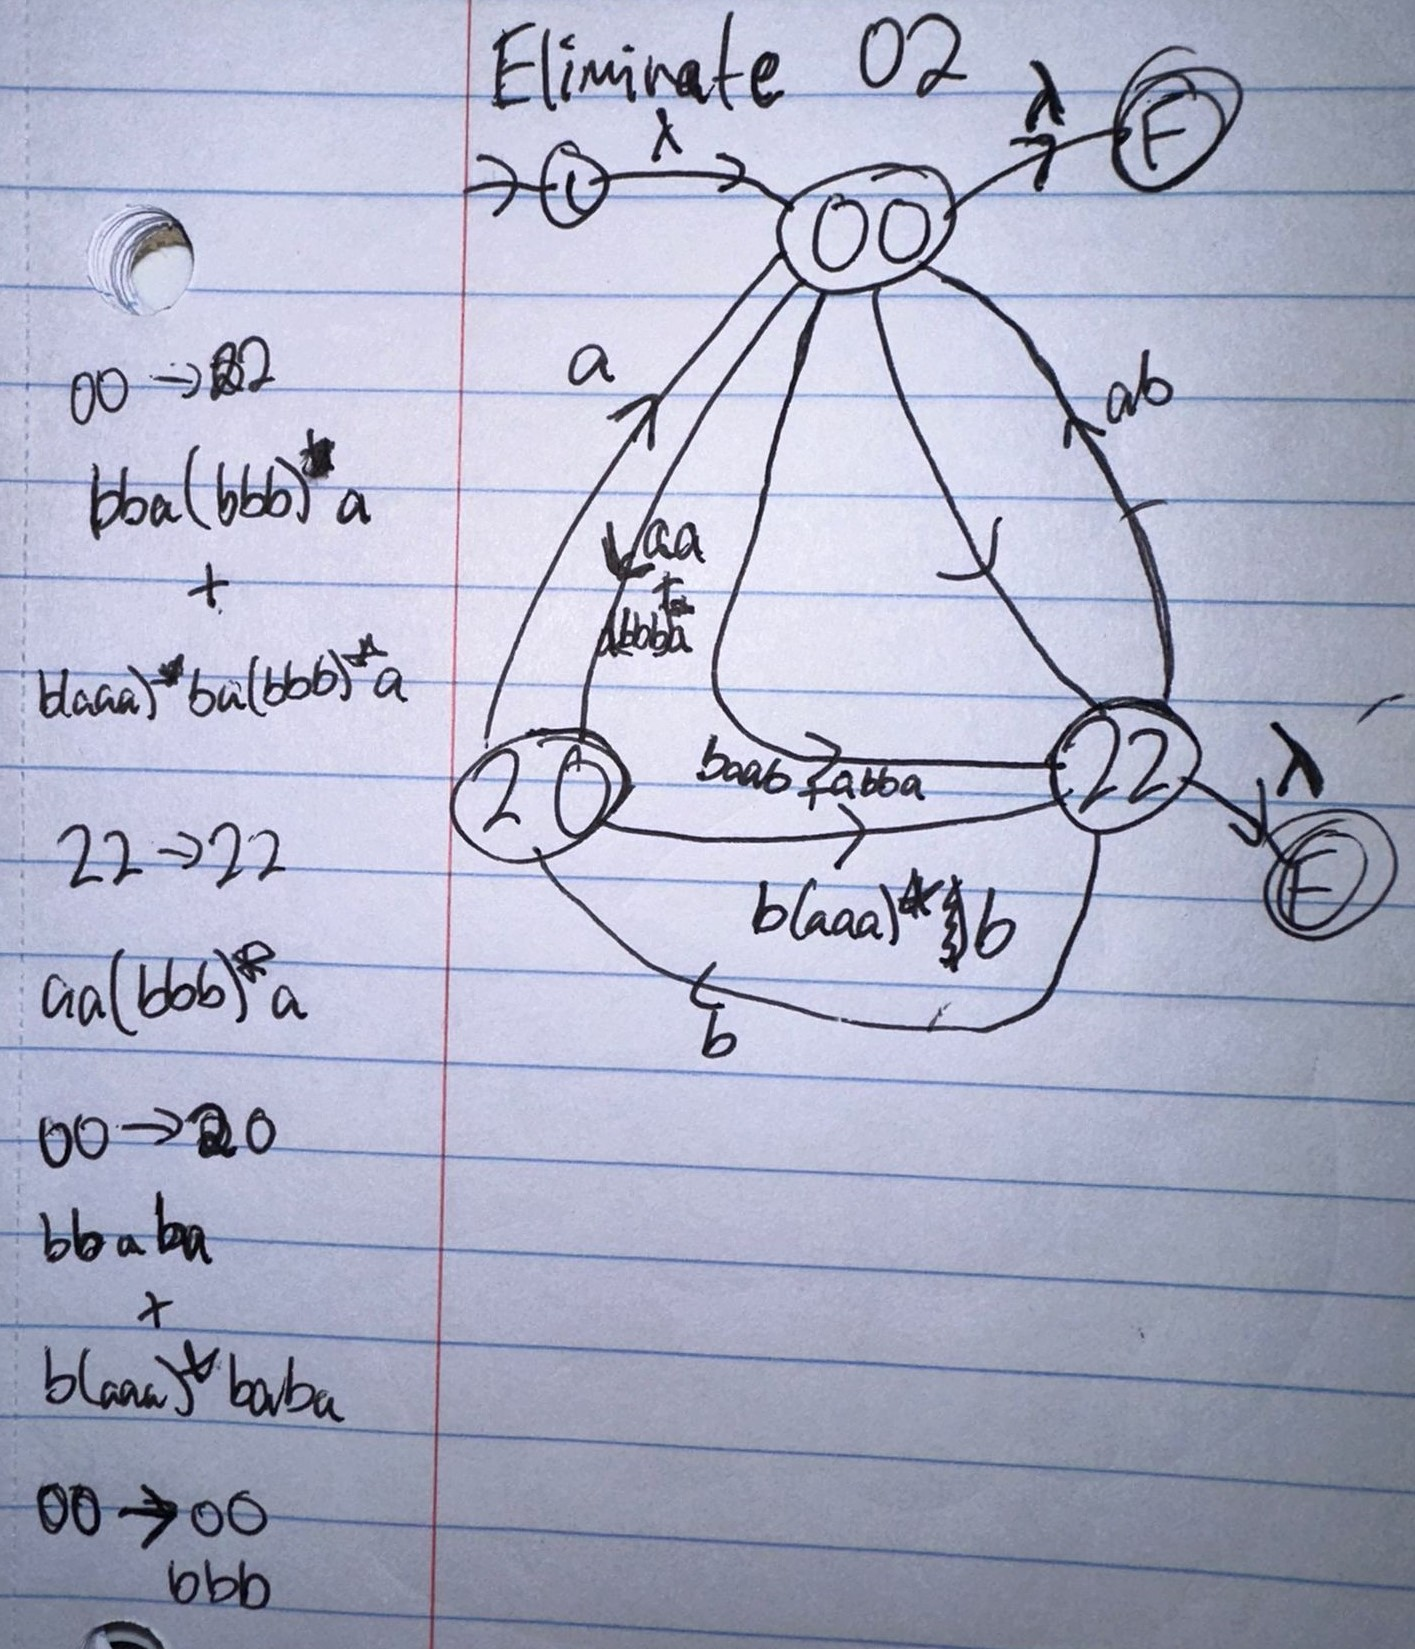
\includegraphics[scale=.2]{14.10.3.7}
	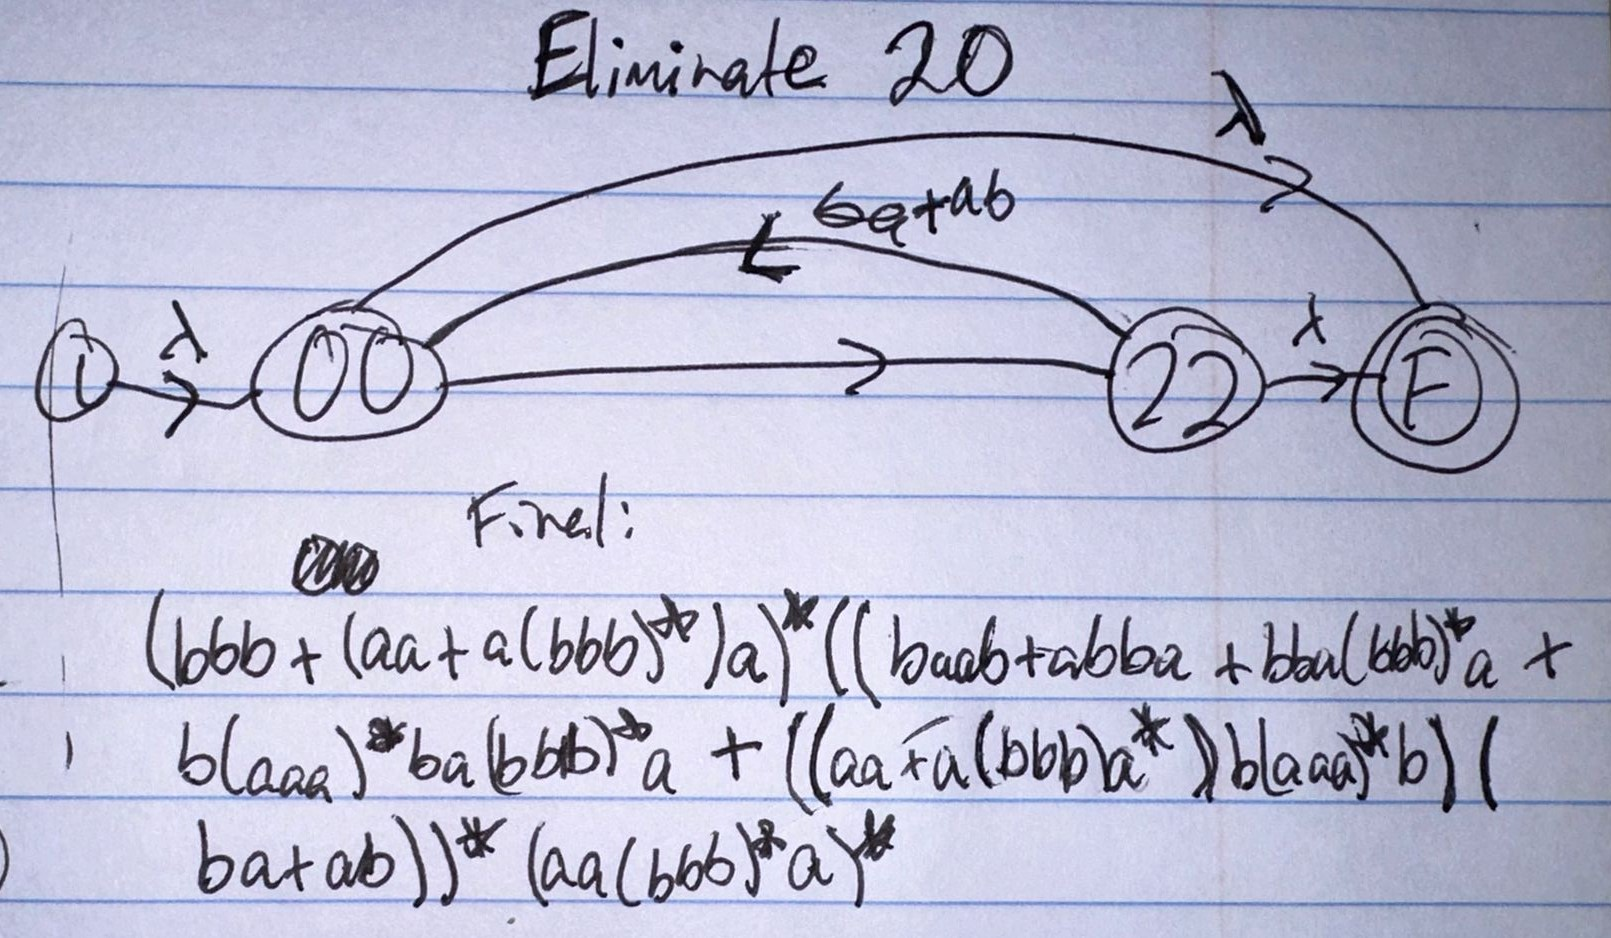
\includegraphics[scale=.2]{14.10.3.8}
\end{figure}

The final regular expression is the following:
\[ ((bbb + (aa + a(bbb)^*)a)^* ((baab+abba+bba(bbb)^*a + b(aaa)^*ba(bbb)^*a) + ((aa + \]
\[a(bbb)^*a)b(aaa)^*b) (ba + ab))^* (aa(bbb)^*a)^*)^* \]


\newpage
\section*{\textbf{EC: P15.6.2} [10 pts]}
Build a Turing machine $M_{copy}$ that when started on input $w$ (i.e., in configuration $\iota \square w$), halts with the tape contents $\square w \square w$. (Here $i$ is the start state.) You need not give the entire state table as long as your description is clear and complete. Let $\Sigma = \{a, b\}$.

\subsection*{\textbf{Solution:}}
For this machine, $\Gamma = \{ a, b, \alpha, \beta, \square \} $ \\

To give a broad overview, this machine iteratively copies the letters of the first string $w$ to the end. It will see a letter, then move to the end and print that letter, than move back to read the next letter. It keeps doing this until all letters have been copied. The machine keeps track of which letters have already been copied by replacing them with $\alpha$ if it was $a$ or $\beta$ if it was $b$. The machine then replaces all of these stand-in characters at the end to ensure the strings match the original. \\

It will start in the state $\iota$ and upon seeing $\square$ it will print $\square$ and move right while staying in $\iota$.

If it sees an $a$, it will enter the "read a" state and print $\alpha$, then continuously move right while not printing anything and remain in the same state until it sees a $\square$. Then it will move to the "print a" state and continue moving right without printing. 

If it sees a $b$, it will enter the "read b" state and print $\beta$, then continuously move right while not printing anything and remain in the same state until it sees a $\square$. Then it will move to the "print b" state and continue moving right without printing. 

When it sees a $\square$ it will print $a$ or $b$ based on whether it was in "print a" or "print b" then enter the "reverse second" state and start moving left. When it sees $\square$ it will enter the "reverse first" state and keep moving left. 

When it sees either $\alpha$ or $\beta$ it will move right. If $a$ is seen it goes back to "read a" and if it's $b$ it goes back to "read b" and the process repeats.

If "reverse first" does not encounter an $a$ or $b$ past the $\square$ buffer it knows all the original characters have been replaced by $alpha$ or $beta$ which means the string has been successfully copied. Now it must move back to the beginning $\square$ and go one by one replacing the characters.

We can have a state called "replace first" and "replace second". "replace second" just needs to traverse to the beginning of the second string without printing or changing state by moving left. If it sees $\square$ it will change state to "replace first" which will print $a$ if it sees $\alpha$ or $b$ if it sees $\beta$ then move left. Once "replace first" reaches $\square$ everything will have been replaced so we move to the "halt" state and the string will now have been copied.


\end{document} 